\section{Zielsetzung}
\label{sec:Zielsetzung}
Ziel dieses Versuch ist es den Lock-In-Verstärker zu verstehen und dessen Funktionsweise.

\section{Theorie}
\label{sec:Theorie}
 \subsection{Allgemein} % (fold)
 \label{sub:Allgemein}
 Der Lock-In-Verstärker ist, wie der Name schon sagt, ein Verstärker, in dem ein phasenempfindlicher Detektor intgriert ist.
 Er wird hauptsächlich für die Messung verrauschter Signale benutzt, wobei das Messsignal mit einer Referenzsignal $\omega_0$ moduliert wird.
 \begin{figure}[H]
    \centering
    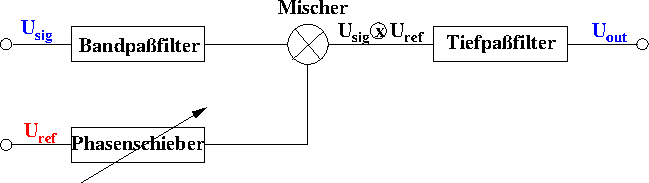
\includegraphics[width=0.5\textwidth]{build/Abb_1.pdf}
    \caption {Schematische Darstellung eines Lock-In-Verstärkers.[1]\cite{v303}}
    \label{fig:Abb_1}
\end{figure}
Im Folgenden wir der Lock-In-Verstärker schematisch mit \autoref{fig:Abb_2} erklärt.
Das Nutzsignal $U_sig$, was moduliert und verrauscht ist, wird durch ein Bandpassfilter zu einem Mischer geleitet.
Der Bandpassfilter befreit das Signal von Frequnezen, die viel größer sind als die Referenzfrequenz $(\omega >> \omega_0)$ und die viel kleiner $(\omega << \omega_0)$ sind.
Außerdem wird eine Referenzsignal $U_ref$ durch einen Phasenschieber zum Mischer geleitet.
Mit dem Phasenschieber kann die Phase des Referenzsignals variiert werden und mit dem Nutzsignal synchronisiert werden.
 
 % subsection Allgemein (end)
